\chapter{Tight binding model in the honeycomb lattice}
\label{APD}

Graphene, as a representative two dimensional solid with honeycomb lattice structure has some interesting electrical properties induced by its lattice structure. Graphene is a zero gap semiconductor, meaning that its conduction and valence bands touch each other at the $\bs{K}$ points in the momentum space. Around these points the electrons have a linear dispersion relation, resembling that of massless Dirac fermions. In the following we will show this in detail.

Using the same notation introduced in \ref{AP1A} we can introduce the fermionic operators $\hat{a}^\dagger_i$ and $\hat{b}^\dagger_j$ which create and electron on the A and B site receptively, at position $\bs{R}_i$ or $\bs{R}_i$. Then, the tight binding Hamiltonian considering only NN hopping is:

\begin{equation}
\label{TBHex}
\hat{H} = -t\sum_{i \in A}\sum_{\bs{\delta}} (\hat{a}^\dagger_i\hat{b}_{i+\bs{\delta}} + \hat{b}^\dagger_{i+\bs{\delta}}\hat{a}_i)
\end{equation}

Where $i$ labels sites in sublattice A and $\bs{\delta}$ are the NN vectors, we make an abuse of notation by summing $i+\bs{\delta}$ referring, of course, to the site at position $\bs{R}_i+\bs{\delta}$. In order to diagonalize this Hamiltonian we change to momentum space:

\begin{align}
\hat{a}^\dagger_i &= \frac{1}{\sqrt{N}} \sum_{\bs{k}} e^{i\bs{k}\cdot\bs{r}_i}\hat{a}^\dagger_{\bs{k}} \\
\hat{b}^\dagger_j &= \frac{1}{\sqrt{N}} \sum_{\bs{k}} e^{i\bs{k}\cdot\bs{r}_j}\hat{b}^\dagger_{\bs{k}} 
\end{align}

Then \ref{TBHex} reads:

\begin{align*}
\hat{H} &= -\frac{t}{N} \sum_{i \in A}\sum_{\bs{\delta}} \sum_{\bs{k}\bs{k}'} e^{i(\bs{k}-\bs{k}')\cdot\bs{r}_i}e^{-i\bs{k}'\cdot\bs{\delta}} \hat{a}^\dagger_{\bs{k}}\hat{b}_{\bs{k}'} + e^{i(\bs{k}'-\bs{k})\cdot\bs{r}_i}e^{i\bs{k}'\cdot\bs{\delta}} \hat{b}^\dagger_{\bs{k}'}\hat{a}_{\bs{k}} = \\
&= -t \sum_{\bs{\delta}\bs{k}} e^{-i\bs{k}\cdot\bs{\delta}} \hat{a}^\dagger_{\bs{k}}\hat{b}_{\bs{k}} +e^{i\bs{k}\cdot\bs{\delta}} \hat{b}^\dagger_{\bs{k}}\hat{a}_{\bs{k}} = \sum_{\bs{k}} \psi^\dagger(\bs{k})h(\bs{k})\psi(\bs{k})
\end{align*}

Where $\psi(\bs{k}) = \left( \hat{a}_{\bs{k}}, \hat{b}_{\bs{k}} \right)^T$ and:

\begin{equation}
h(\bs{k}) = \begin{pmatrix}
    0 & f(\bs{k}) \\
    f^*(\bs{k}) & 0
\end{pmatrix}
\end{equation}

being $f(\bs{k}) = -t\sum_{\bs{\delta}} e^{i\bs{k}\cdot\bs{\delta}}$. In order to obtain the band structure we need to diagonalize $h(\bs{k})$. This is straightforward and the resulting energy bands are:

\begin{equation}
E(\bs{k})_{\pm} = \pm|f(\bs{k})| = \pm t\sqrt{3+2\cos(\sqrt{3}k_ya) +4\cos(\sqrt{3}k_y\frac{a}{2})\cos(3k_x\frac{a}{2})}
\end{equation}

The bands will cross, or equivalently the band gap will vanish if $f(\bs{k})=0$ has a solution, which it does at the corners of the first Brillouin zone, i.e. the points:

\begin{align*}
\bs{K} &= \frac{2\pi}{3a}\left( 1, \frac{1}{\sqrt{3}}\right) \\
\bs{K}' &= \frac{2\pi}{3a}\left( 1, -\frac{1}{\sqrt{3}}\right) 
\end{align*}

Where $a$ is the lattice constant. The other corner points are equivalent to either one of these (that is, they can be obtained by a translation of a reciprocal lattice vector).

\begin{figure}
\centering
  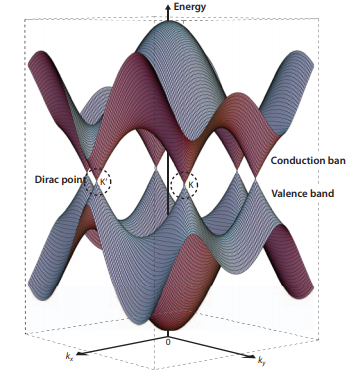
\includegraphics[width=0.7\linewidth]{../Figures/graphene_bands.png}
  \caption{Image from \cite{Ando2009}. The energy bands of graphene.} 
\label{FigD1}
\end{figure}

As depicted in \ref{FigD1} the bands touch in the $\bs{K}$ and $\bs{K}'$ points of the first Brillouin zone. Now, since the system has one electron per atom with two possible spin states it is clear that at zero temperature the lower energy band will be filled (and the upper band will be empty). Thus, the excitations of the system will occur near the crossings at the $\bs{K}$ points. In order to study these excitations it is interesting to linearize the Hamiltonian around these points. Around the $\bs{K}$ point for example, since $f(bs{k})$ vanishes, we can write:

\begin{equation}
h(\bs{K}+\bs{q}) \approx \begin{pmatrix}
    0 & \frac{\partial f(\bs{k})}{\partial \bs{k}}(\bs{K})\bs{q} \\
    \frac{\partial f^*(\bs{k})}{\partial \bs{k}}(\bs{K})\bs{q} & 0
\end{pmatrix}
\end{equation}

Now, 

\begin{equation}
\frac{\partial f(\bs{k})}{\partial \bs{k}}(\bs{K})\bs{q} = -ie^{\frac{2\pi i}{3}} \frac{3a}{2}(q_x+iq_y)
\end{equation}

We can ignore the phase and write:

\begin{equation}
h(\bs{K}+\bs{q}) = v_F \begin{pmatrix}
    0 & q_x+iq_y \\
    q_x-iq_y & 0
\end{pmatrix}
\end{equation}

Where $v_F = \frac{3at}{2}$. This result is usually written in terms of Pauli matrices as:

\begin{equation}
h(\bs{K}+\bs{q}) = v_F(q_x\sigma_x-q_y\sigma_y)
\end{equation}
